
%%%%%%%%%%%%%%%%%%%%%%%%%%%%%%%%%%%%%%%%%%%%%%%%%%%%%%%%%%%
\section{Object Manipulation With Hardware Robots}\label{sec:realExperiment}
%%%%%%%%%%%%%%%%%%%%%%%%%%%%%%%%%%%%%%%%%%%%%%%%%%%%%%%%%%%

  
\subsection{Environmental Setup}
Our experiments are on centimeter-scale hardware systems called \emph{kilobots}.  These allows us to emulate a variety of dynamics, while enabling a high degree of control over robot function, the environment, and data collection. The kilobot \cite{Rubenstein2012,rubenstein2014programmable} is a low-cost robot designed for testing collective algorithms with large numbers of robots. It is available commercially or as an open source platform~\cite{K-Team2015}.  Each robot is approximately 3 cm in diameter, 3 cm tall, and uses two vibration motors to move on a flat surface at speeds up to 1 cm/s.  Each robot has one ambient light sensor that is used to implement \emph{phototaxis},  moving towards a light source. 
In these experiments as shown in Fig.~\ref{fig:setup}, we used $n$=64 kilobots, a 1.5 m$\times$1.2 m whiteboard as the workspace, and four 30W LED floodlights arranged 1.5 m above the plane of the table at the $\{N,E,S,W\}$ vertices of a 6 m square centered on the workspace. The lights were controlled using an Arduino Uno board connected to an 8 relay shield board.  At top of the table, an overhead machine vision system was added to track the position of the swarm. Laser-cut patterns for our neon green fiducial markers and our {\sc Matlab} tracking code are available at our github repository~\cite{Shahrokhi2015GitHubShapeControl}.
\begin{figure}
\begin{center}
	\includegraphics[width=\columnwidth]{SetUp.jpg}
\end{center}
\caption{\label{fig:setup}
Hardware platform:  table with 1.5$\times$1.2 m workspace, surrounded by four remotely triggered 30W LED floodlights, with an overhead machine vision system.
}
\end{figure}
\subsection{Mean Control With Real Robots}

\begin{figure}
\begin{center}
	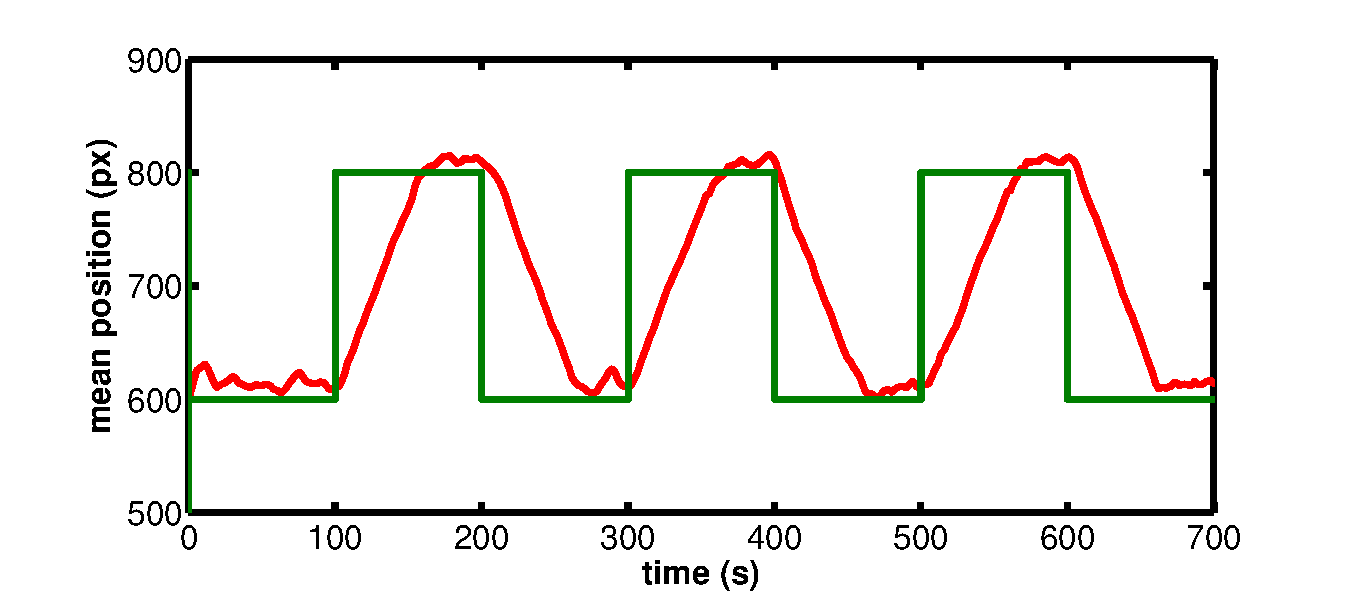
\includegraphics[width=\columnwidth]{Mean_Control_experiment.eps}
\end{center}
\caption{\label{fig:realMean}
Mean Control plot with kilobots.
}
\end{figure}

\begin{figure}
\begin{center}
	\includegraphics[width=\columnwidth]{XYMeanControl.eps}
\end{center}
\caption{\label{fig:meanRobotFig}
Mean Control experiment with kilobots.
}
\end{figure}

\subsection{Automated Object Manipulation}


\begin{figure}
\centering
\begin{overpic}[width=1\columnwidth]{BlockBotView2.eps}\end{overpic}
%\todo{I like the 'target' symbol, but it is not self-documenting.  We need a legend explaining the min and max variance ellipses, the goal region, the variance, the mean, the object COM, and the target mean position.  I think these are easiest to make in powerpoint.
%Please use the same color and line style for the variance min and max as you use in Figure 4.
%}
%{blockpushingImageWithMeanAndVarianceOverlay.png}
\caption{\label{fig:bigPictureMeanAndVarianceForSwarm} A swarm of robots, all controlled by a uniform force field, can be effectively controlled by a hybrid controller that knows only the first and second moments of the robot distribution.  Here is a mockup of a swarm of hardware robots(kilobots) that pushes a green block toward the goal. See video attachment~\cite{ShivaVideo2015}.}
\end{figure}